\subsection{Die Grafischen Oberflächen}

Teil der Grafischen Oberfläche ist das Spielfeld (\autoref{fig:gui-tiles}), mit dem die Nutzer wie im Konzept beschrieben, interagieren. Es stellt nicht nur die einzelnen Töne als quadratische Flächen dar, sondern dient auch als Informationsfeld (siehe auch \autoref{ssec:CtA}). Die Tiles können ihre Farbe wechseln und haben verschiedene Animationen. Näheres hierzu kann in \autoref{sec:tiles} nachgelesen werden.

\begin{figure}[htbp] 
  \centering
     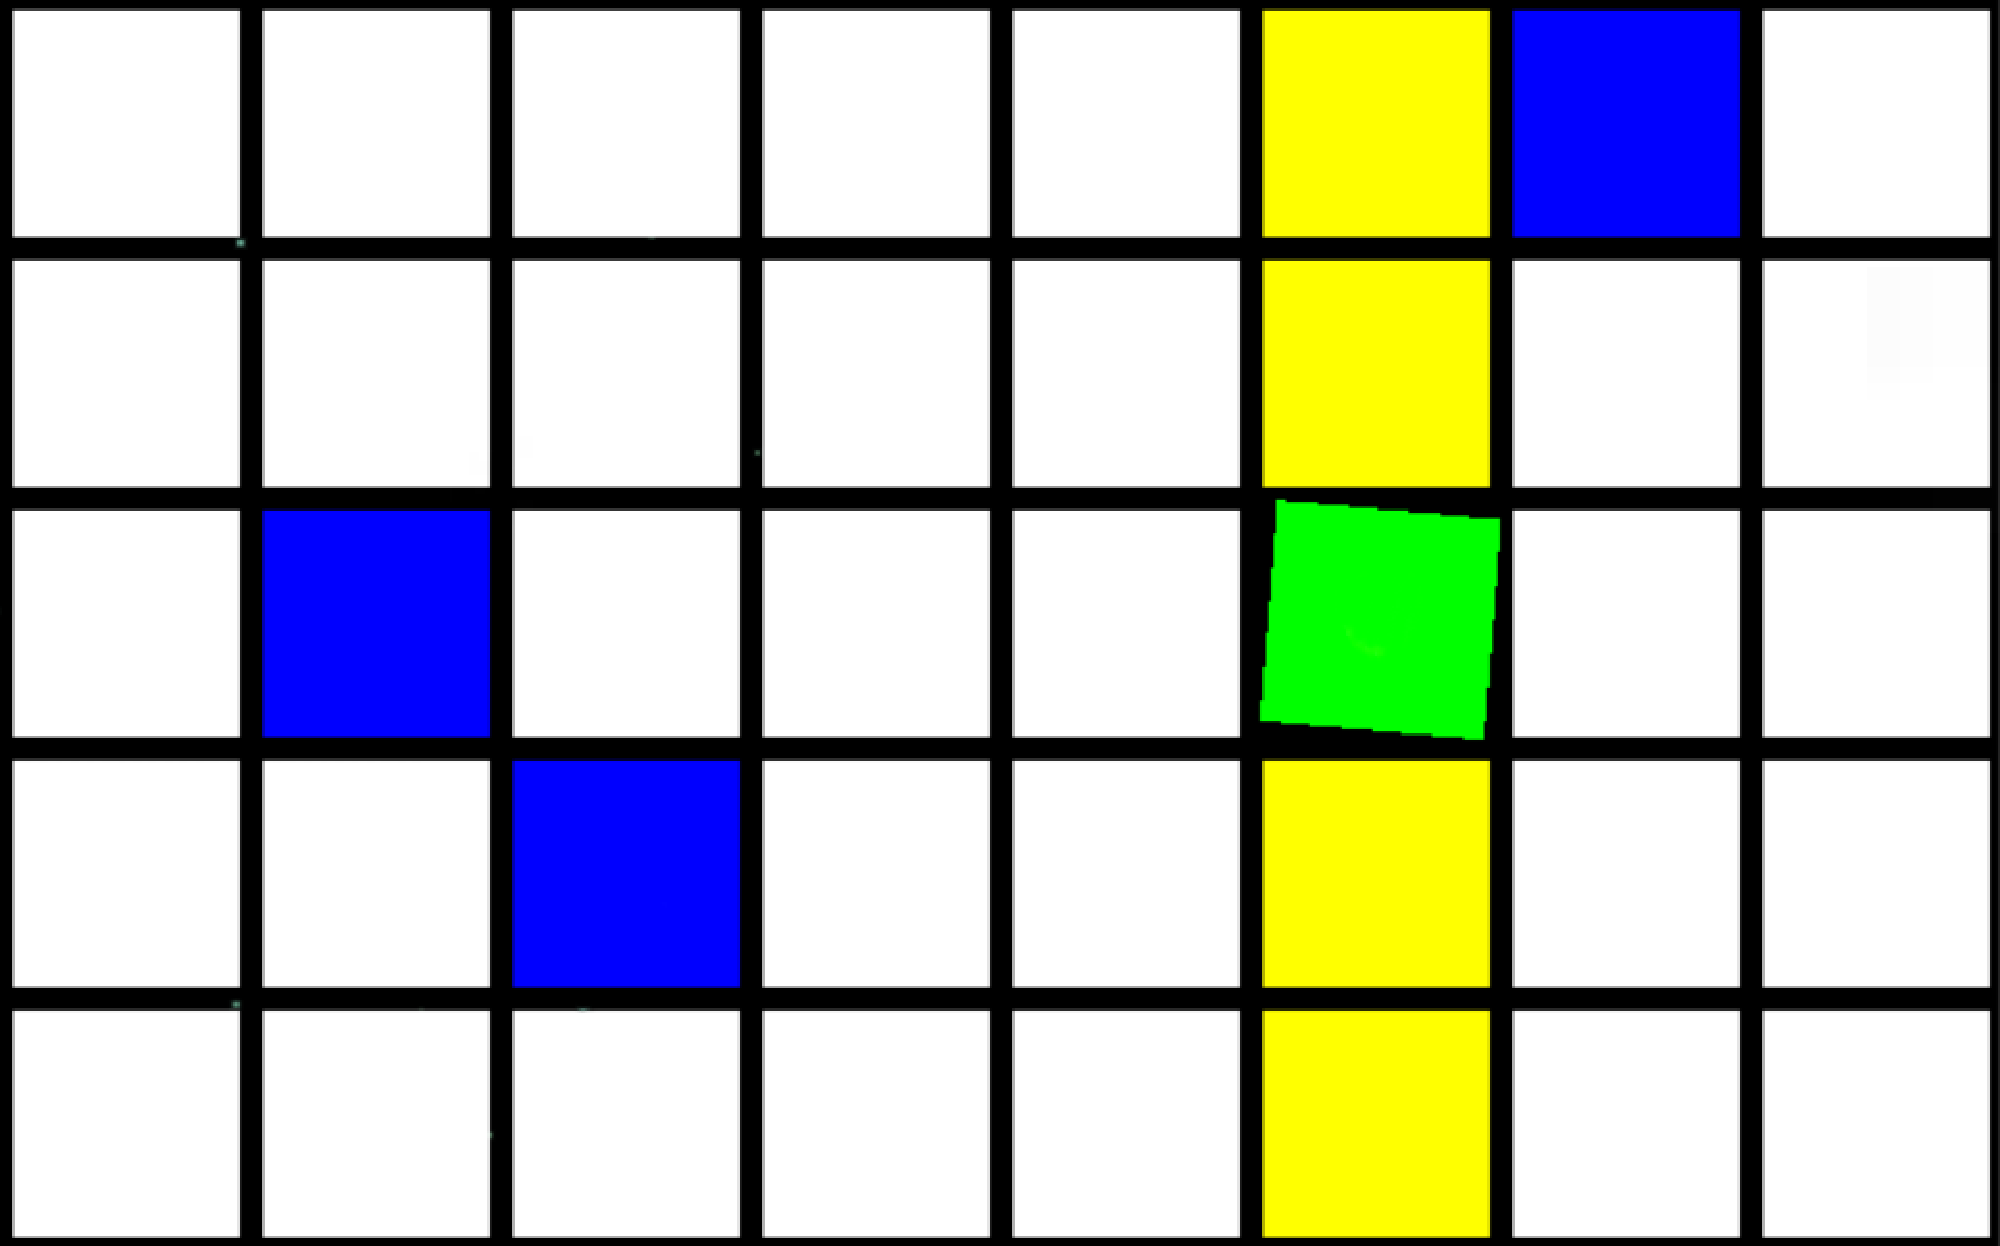
\includegraphics[width=0.9\textwidth]{images/gui-tiles}
  \caption{Das Spielfeld}
  \label{fig:gui-tiles}
\end{figure}

Neben dem Spielfeld wurde für die Bildverarbeitung der BlinkenTiles Anwendung eine weitere Bedienoberfläche entwickelt (siehe Abbildung \autoref{fig:blob}). Sie liegt auf dem linken Bildschirm und kann so nur auf dem PC-Bildschirm eingesehen werden, während der rechte Bildschirm das Spielfeld darstellt und vom Beamer auf den Boden projiziert wird. Die Einstellungen ermöglichen unter anderem die Kalibrierung der Kinect und die Abstimmung mit der tatsächlichen Spielfeldgröße. Näheres hierzu findet sich in \autoref{sec:objdet}.\\
Eine dritte grafische Oberfläche wurde für den Presentation-Screen entwickelt, siehe hierzu \autoref{ssec:CtA}.

\begin{figure}[htbp] 
  \centering
     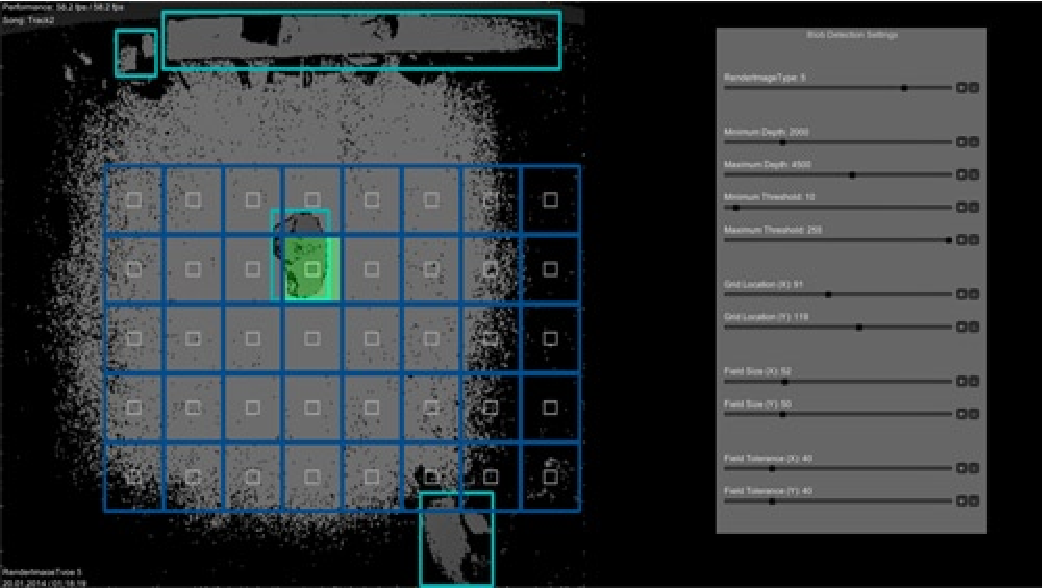
\includegraphics[width=0.9\textwidth]{images/Blob}
  \caption{GUI für die Bildverarbeitung}
  \label{fig:blob}
\end{figure}
